
\begin{figure}[h]
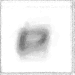
\includegraphics{building-mean}
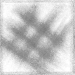
\includegraphics{dirt-mean}
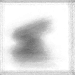
\includegraphics{forest-mean}
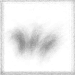
\includegraphics{grass-mean}
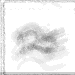
\includegraphics{water-mean}
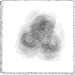
\includegraphics{rocks-mean}
\caption{Mean gold images for buildings, dirt, forest, grass, water, and rocks}
\label{figure:means}
\end{figure}


Gold comparison works by comparing a candidate image, $A$ to a gold standard
image $G$ representing a possible class of $A$. If $A$ is similar to $G$, then
there is a high probability that $A$ belongs to the class which $G$ represents.
Before comparing the images, we need to make the symbols $A$ and $G$ overlap so
that we can more accurately compare pixel-to-pixel.  To overlap the images, we
define $x$ and $y$ to be the row and column sums of the image and calculate the
mean and standard deviation of $x$ and $y$, similar to the feature based
approach. To get the symbols to overlap we apply a linear transformation to
each pixel using the statistics gathered in each dimension.

\[
\label{eq:gold}
x^{\prime} = (x - \mu^{A}_{x}) \, \frac{\sigma^{G}_{x}}{\sigma^{C}_{x}} + \mu^{G}_{x}
\quad\quad\quad
y^{\prime} = (y - \mu^{A}_{y}) \, \frac{\sigma^{G}_{y}}{\sigma^{C}_{y}} + \mu^{G}_{y}
\]

These new transformed pixels replace those in the image $A$ which now overlap
with those in the gold image $G$. We then compare the overlapping image $A$ to
the gold standard image $G$ by taking the sum of the squared difference at each
pixel position. This gives us an error measure, which we record for each of the
$k$ classes.

\[ \xi_{k}(A) = \sum_{i}\sum_{j}{(A_{ij} - G_{kij})^{2}} \]

The result is a vector, $\xi$ with an error measure for the comparison against
each class. For training purposes, we then input this vector into WEKA along
with the correct answer.

To create the gold images, we collect all the samples in our data set and
create a mean gold image by overlapping all the samples belonging to the same
class, the results can be seen in Figure \ref{figure:means} on page
\pageref{figure:means}.
